\bta{测定物体的加速度}
\begin{enumerate}
\renewcommand{\labelenumi}{\arabic{enumi}.}
% A(\Alph) a(\alph) I(\Roman) i(\roman) 1(\arabic)
%设定全局标号series=example	%引用全局变量resume=example
%[topsep=-0.3em,parsep=-0.3em,itemsep=-0.3em,partopsep=-0.3em]
%可使用leftmargin调整列表环境左边的空白长度 [leftmargin=0em]
\item
\exwhere{$ 2019 $ 年全国\lmd{1}卷}
某小组利用打点计时器对物块沿倾斜的长木板加速下滑时的运动进行研究。
物块拖动纸带下滑,打出的纸带一部分如图所示。已知打点计时器所用交流电的频率为 $ 50 \ Hz $,纸
带上标出的每两个相邻点之间还有 $ 4 $ 个打出的点未画出。在 $ ABCDE $ 五个点中,打点计时器最先打
出的是 \tk{A} 点,在打出 $ C $ 点时物块的速度大小为
\tk{$ 0.233 $} 
$ m/s $(保留 $ 3 $ 位有效数字);物块下滑的
加速度大小为
\tk{$ 0.75 $} 
$ m/s^{2} $(保留 $ 2 $ 位有效数字)。
\begin{figure}[h!]
\centering
\includesvg[width=0.83\linewidth]{picture/svg/GZ-3-tiyou-0418}
\end{figure}

\banswer{

}

\item 
\exwhere{$ 2017 $ 年新课标 \lmd{1} 卷}
某探究小组为了研究小车在桌面上的直线运动,用自制“滴水计时器”计量时间。实验前,将该计时
器固定在小车旁,如图($ a $)所示。实验时学.科.网,保持桌面水平,用手轻推一下小车。在小车运
动过程中,滴水计时器等时间间隔地滴下小水滴,图($ b $)记录了桌面上连续的 $ 6 $ 个水滴的位置。
(已
知滴水计时器每 $ 30 \ s $ 内共滴下 $ 46 $ 个小水滴)
\begin{figure}[h!]
\centering
\includesvg[width=0.83\linewidth]{picture/svg/GZ-3-tiyou-0420}
\end{figure}






\begin{enumerate}
\renewcommand{\labelenumi}{\arabic{enumi}.}
% A(\Alph) a(\alph) I(\Roman) i(\roman) 1(\arabic)
%设定全局标号series=example	%引用全局变量resume=example
%[topsep=-0.3em,parsep=-0.3em,itemsep=-0.3em,partopsep=-0.3em]
%可使用leftmargin调整列表环境左边的空白长度 [leftmargin=0em]
\item
由图($ b $)可知,小车在桌面上是 \tk{从右向左} (填“从右向左”或“从左向右”)运动的。
\item 
该小组同学根据图($ b $)的数据判断出小车做匀变速运动。小车运动到图($ b $)中 $ A $ 点位置时
的速度大小为 \tk{$ 0.19 $} $ m/s $,加速度大小为 \tk{$ 0.037 $} $ m/s^{2} $。
(结果均保留 $ 2 $ 位有效数字)




\end{enumerate}

\banswer{

}


\newpage
\item 
\exwhere{$ 2016 $ 年天津卷}
某同学利用图示装置研究小车的匀变速直线运动
\begin{figure}[h!]
\centering
\includesvg[width=0.43\linewidth]{picture/svg/GZ-3-tiyou-0421}
\end{figure}

①实验中必要的措施是 \tk{AB} 

\fourchoices
{细线必须与长木板平行}
{先接通电源再释放小车}
{小车的质量远大于钩码的质量}
{平衡小车与长木板间的摩擦力}

②他实验时将打点计时器接到频率为 $ 50 \ HZ $ 的交流电
源上,得到一条纸带,打出的部分计数点如图所示(每相邻两个计数点间还有 $ 4 $ 个点,图中未画出);
$ s_{1}=3.59 \ cm $;$ s_{2}=4.41 \ cm $;$ s_{3}=5.19 \ cm $;
$ s_4=5.97 \ cm $;$ s_5=6.78 \ cm $;$ s_6=7.64 \ cm $;
则小车的加速度 $ a= $
\tk{$ 0.80 $} 
$ m/s $ (要求
充分利用测量数据),打点计时器在打 $ B $ 点时小车的速度 $ v_{B} = $
\tk{0.40} 
$ m/s $;
(结果均保留两位有效数
字)
\begin{figure}[h!]
\centering
\includesvg[width=0.63\linewidth]{picture/svg/GZ-3-tiyou-0422}
\end{figure}





\item 
\exwhere{$ 2016 $ 年海南卷}
某同学利用图($ a $)所示的实验装置探究物块速度随时间的变化。物块放在桌面
上,细绳的一端与物块相连,另一端跨过滑轮挂上钩码。打点计时器固定在桌面左端,所用交流电
源频率为 $ 50 \ Hz $。纸带穿过打点计时器连接在物块上。启动打点计时器,释放物块,物块在钩码的
作用下拖着纸带运动。打点计时器打出的纸带如图($ b $)所示(图中相邻两点间有 $ 4 $ 个点未画出)。
\begin{figure}[h!]
\centering
\includesvg[width=0.83\linewidth]{picture/svg/GZ-3-tiyou-0423}
\end{figure}




根据实验数据分析,该同学认为物块的运动为匀加速运动。回答下列问题:
\begin{enumerate}
\renewcommand{\labelenumi}{\arabic{enumi}.}
% A(\Alph) a(\alph) I(\Roman) i(\roman) 1(\arabic)
%设定全局标号series=example	%引用全局变量resume=example
%[topsep=-0.3em,parsep=-0.3em,itemsep=-0.3em,partopsep=-0.3em]
%可使用leftmargin调整列表环境左边的空白长度 [leftmargin=0em]
\item
在打点计时器打出 $ B $ 点时,物块的速度大小为 \tk{$ 0.56 $} $ m/s $。在打出 $ D $ 点时,物块的速度大小为 \tk{$ 0.96 $} 
$ m/s $;
(保留两位有效数字)
\item 
物块的加速度大小为 \tk{$ 2.0 $} $ m/s $。(保留两位有效数字)




\end{enumerate}



\newpage
\item
\exwhere{$ 2011 $ 年理综广东卷}
\begin{enumerate}
\renewcommand{\labelenumi}{\arabic{enumi}.}
% A(\Alph) a(\alph) I(\Roman) i(\roman) 1(\arabic)
%设定全局标号series=example	%引用全局变量resume=example
%[topsep=-0.3em,parsep=-0.3em,itemsep=-0.3em,partopsep=-0.3em]
%可使用leftmargin调整列表环境左边的空白长度 [leftmargin=0em]
\item
图$ (a) $是“研究匀变速直线运动”实验中获得的一条纸带,$ O $、$ A $、$ B $、$ C $、$ D $ 和 $ E $ 为纸带上
六个计数点。加速度大小用 $ a $ 表示。

①$ OD $ 间的距离为 \tk{$ 1.20 $} $ cm $。

②图$ (b) $是根据实验数据绘出的 $ s- t^{2} $ 图线($ s $ 为各计数点至同一起点的距离)
,斜率表示 \tk{加速度一半,} ,其
大小为 \tk{$ 0.933 $} $ m/s^{2} $(保留三位有效数字)。


\end{enumerate}
\begin{figure}[h!]
\centering 
\includesvg[width=0.8\linewidth]{picture/svg/GZ-3-tiyou-0424}
\end{figure}

\banswer{

}



\item
\exwhere{$ 2014 $ 年理综大纲卷}
现用频闪照相方法来研究物块的变速运动。在一小物块沿斜面向下运动的过程中,用频
闪相机拍摄的不同时刻物块的位置如图所示。拍摄时频
闪频率是 $ 10 \ Hz $;通过斜面上固定的刻度尺读取的 $ 5 $ 个连
续影像间的距离依次为 $ x_{1} $、$ x_{2} $、$ x_{3} $、$ x_{4} $。已知斜面顶端的
高度 $ h $ 和斜面的长度 $ s $。数据如下表所示(单位:$ cm $)。重力加速度
大小 $ g=9.80 \ m/s^{2} $。
% TODO: \usepackage{graphicx} required
\begin{figure}[h!]
\centering
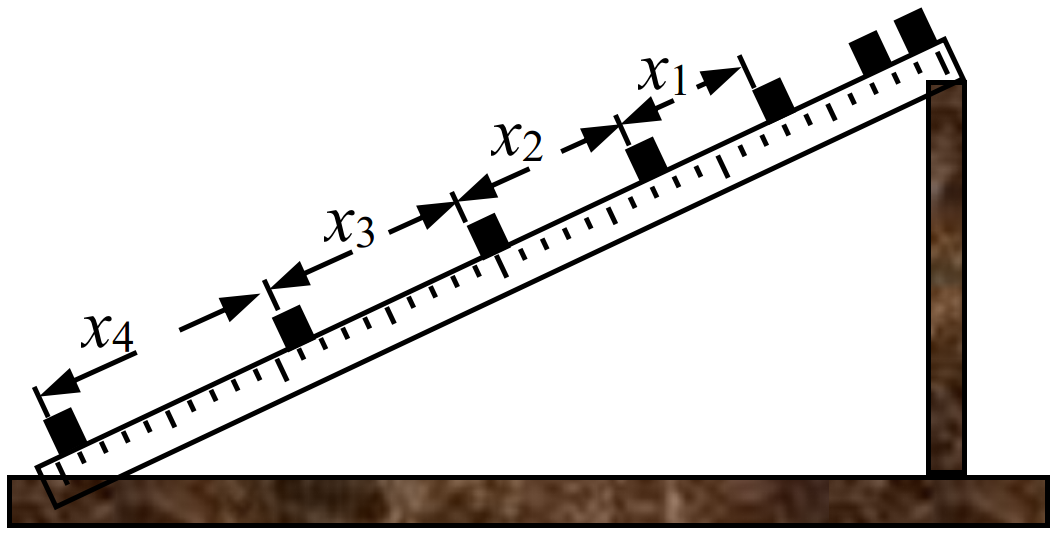
\includegraphics[width=0.43\linewidth]{picture/screenshot030}
\end{figure}




\begin{table}[h!]
\centering 
\begin{tabular}{|c|c|c|c|c|c|}
\hline$x_{1}$ & $x_{2}$ & $x_{3}$ & $x_{4}$ & $h$ & $s$ \\
\hline 10.76 & 15.05 & 19.34 & 23.65 & 48.00 & 80.00 \\
\hline
\end{tabular}
\end{table} 


根据表中数据,完成下列填空:
\begin{enumerate}
\renewcommand{\labelenumi}{\arabic{enumi}.}
% A(\Alph) a(\alph) I(\Roman) i(\roman) 1(\arabic)
%设定全局标号series=example	%引用全局变量resume=example
%[topsep=-0.3em,parsep=-0.3em,itemsep=-0.3em,partopsep=-0.3em]
%可使用leftmargin调整列表环境左边的空白长度 [leftmargin=0em]
\item 
物块的加速度 $ a= $
\tk{$ 4.30 $(填“$ 4.29 $”或“$ 4.31 $”同样给分)} 
$ m/s_{2} $(保留 $ 3 $ 位有效数字)。

\item 
因为
\tk{物块加速度小于 $ gh/s=5.88 \ m/s^{2} $(或:物块加速度小于物块沿光滑斜面下滑的加速度)} 
,可知斜面
是粗糙的。




\end{enumerate}


\banswer{

}


\newpage
\item 
\exwhere{$ 2013 $ 年广东卷}
研究小车匀变速直线运动的实验装置如图 $ 16 $($ a $)所示,其中斜面倾角$ \theta $可调,打点计时器
的工作频率为 $ 50 \ HZ $,纸带上计数点的间距如图 $ 16 $($ b $)所示,其中每相邻两点之间还有 $ 4 $ 个记录点
未画出。
\begin{figure}[h!]
\centering
\includesvg[width=0.83\linewidth]{picture/svg/GZ-3-tiyou-0426}
\end{figure}



①部分实验步骤如下:

A.测量完毕,关闭电源,取出纸带




B.接通电源,待打点计时器工作稳定后放开小车



C.将小车停靠在打点计时器附近,小车尾部与纸带相连



D.把打点计时器固定在平板上,让纸带穿过限位孔



上述实验步骤的正确顺序是: \tk{$ DCBA $} (用字母填写)。



②图 $ 16 $($ b $)中标出的相邻两计数点的时间间隔 $ T= $
\tk{$ 0.1 $} 
$ s $

③计数点 $ 5 $ 对应的瞬时速度大小计算式为 $ v_5= $
\tk{$\frac{s_{4}+s_{5}}{2 T}$} 
。

④为了充分利用记录数据,减小误差,小车加速度大小的计算式应为 $ a= $ \tk{$\frac{\left(s_{4}+s_{5}+s_{6}\right)-\left(s_{1}+s_{2}+s_{3}\right)}{9 T^{2}}$} 。



\newpage
\item
\exwhere{$ 2018 $年江苏卷}
某同学利用如图所示的实验装置来测量重力加速度$ g $。细绳跨过固定在
铁架台上的轻质滑轮,两端各悬挂一只质量为$ M $的重锤。实验操 作如下:

①用米尺量出重锤$ 1 $底端距地面的高度$ H $;



②在重锤$ 1 $上加上质量为$ m $的小钩码;

③左手将重锤$ 2 $压在地面上,保持系统静止。释放重锤$ 2 $,同时右手开启
秒表,在重锤$ 1 $落地时停止计时,记录下落时间;

④重复测量$ 3 $次下落时间,取其平均值作为测量值$ t $。
\begin{figure}[h!]
\centering
\includesvg[width=0.26\linewidth]{picture/svg/GZ-3-tiyou-0428}
\end{figure}



请回答下列问题:
\begin{enumerate}
\renewcommand{\labelenumi}{\arabic{enumi}.}
% A(\Alph) a(\alph) I(\Roman) i(\roman) 1(\arabic)
%设定全局标号series=example	%引用全局变量resume=example
%[topsep=-0.3em,parsep=-0.3em,itemsep=-0.3em,partopsep=-0.3em]
%可使用leftmargin调整列表环境左边的空白长度 [leftmargin=0em]
\item
步骤④可以减小对下落时间$ t $测量的
\tk{偶然} 
(选填“偶然”或“系统”)误差。

\item 
实验要求小钩码的质量$ m $要比重锤的质量$ M $小很多,主要是为了
\tk{B} 
。

\fourchoices
{使$ H $测得更准确}
{使重锤$ 1 $下落的时间长一些}
{使系统的总质量近似等于$ 2M $}
{使细绳的拉力与小钩码的重力近似相等}

\item 
滑轮的摩擦阻力会引起实验误差。现提供一些橡皮泥用于减小该误差,可以怎么做?

\tk{在重锤 $ 1 $ 上粘上橡皮泥,调整橡皮泥质量直至轻拉重锤 $ 1 $ 能观察到其匀速下落} 

\item 
使用橡皮泥改进实验后,重新进行实验测量,并测出所用橡皮泥的质量为$ m_{0} $。用实验中的测
量量和已知量表示$ g $,得$ g= $ \tk{$\frac{2\left(2 M+m+m_{0}\right) H}{m t^{2}}$} 。


\end{enumerate}



\newpage
\item 
\exwhere{$ 2013 $年江苏卷}
某兴趣小组利用自由落体运动测定重力加速度,实验装置如图所示. 倾斜的球槽中放有若
干个小铁球,闭合开关$ K $,电磁铁吸住第$ 1 $ 个小球. 手动敲击弹性金属片$ M,M $ 与触头瞬间分开, 第$ 1 $
个小球开始下落,$ M $ 迅速恢复,电磁铁又吸住第$ 2 $ 个小球。 当
第$ 1 $ 个小球撞击$ M $ 时,$ M $ 与触头分开,第$ 2 $ 个小球开始下
落$ \cdots \cdots $ 这样,就可测出多个小球下落的总时间.
\begin{figure}[h!]
\centering
\includesvg[width=0.35\linewidth]{picture/svg/GZ-3-tiyou-0429}
\end{figure}


\begin{enumerate}
\renewcommand{\labelenumi}{\arabic{enumi}.}
% A(\Alph) a(\alph) I(\Roman) i(\roman) 1(\arabic)
%设定全局标号series=example	%引用全局变量resume=example
%[topsep=-0.3em,parsep=-0.3em,itemsep=-0.3em,partopsep=-0.3em]
%可使用leftmargin调整列表环境左边的空白长度 [leftmargin=0em]
\item
在实验中,下列做法正确的有 \tk{BD} 
\fourchoices
{电路中的电源只能选用交流电源}
{实验前应将$ M $ 调整到电磁铁的正下方}
{用直尺测量电磁铁下端到$ M $ 的竖直距离作为小球下落的高度}
{手动敲击$ M $ 的同时按下秒表开始计时}


\item 
实验测得小球下落的高度 $ H=1.980 \ m $,$ 10 $ 个小球下落的总时间 $ T=6.5 \ s $. 可求出重力加速度
$ g= $ \tk{$ 9.4 $} $ m/s^{2}. $(结果保留两位有效数字)



\item 
在不增加实验器材的情况下,请提出减小实验误差的两个办法.

\tk{增加小球下落的高度;多次重复实验,结果取平均值.(其他答案只要合理也可)} 

\item 
某同学考虑到电磁铁在每次断电后需要时间$ \Delta t $ 磁性才消失,因此,每个小球的实际下落时间与它
的测量时间相差$ \Delta t $,这导致实验误差. 为此,他分别取高度$ H_{1} $ 和$ H_{2} $,测量$ n $个小球下落的总时间$ T_{1} $ 和$ T_{2} $.
他是否可以利用这两组数据消除$ \Delta t $ 对实验结果的影响? 请推导说明.


\banswer{
由$H_{1}=\frac{1}{2} g\left(\frac{T_{1}}{n}-\Delta t\right)^{2}$ 和 $H_{2}=\frac{1}{2} g\left(\frac{T_{2}}{n}-\Delta t\right)^{2}$
\\
可得 $g=\frac{2 n^{2}(\sqrt{H_{1}}-\sqrt{H_{2}})^{2}}{\left(T_{1}-T_{2}\right)^{2}},$ 因此可以消去 $\Delta t$ 的影响
}


\end{enumerate}



\newpage
\item 
\exwhere{$ 2012 $年理综山东卷}
某同学利用图甲所示的实验装置,探究物块在水平桌面上的运动规律。物块在重物的牵引下
开始运动,重物落地后,物块再运动一段距离停在桌面上(尚未到达滑轮处)
。从纸带上便于测量
的点开始,每$ 5 $个点取$ 1 $个计数点,相邻计数点间的距离如图乙所示。打点计时器电源的频率为$ 50 \ Hz $。
\begin{figure}[h!]
\centering
\includesvg[width=0.83\linewidth]{picture/svg/GZ-3-tiyou-0430}
\end{figure}


\begin{enumerate}
\renewcommand{\labelenumi}{\arabic{enumi}.}
% A(\Alph) a(\alph) I(\Roman) i(\roman) 1(\arabic)
%设定全局标号series=example	%引用全局变量resume=example
%[topsep=-0.3em,parsep=-0.3em,itemsep=-0.3em,partopsep=-0.3em]
%可使用leftmargin调整列表环境左边的空白长度 [leftmargin=0em]
\item
通过分析纸带数据,可判断物块在相邻计数点
\tk{$ 6 $} 
和
\tk{$ 7 $} 
之间某时刻开始减速。


\item 
计数点$ 5 $对应的速度大小为
\tk{1.00} 
$ m/s $,计数点$ 6 $对应的速度大小为
\tk{$ 1.20 $} 
$ m/s $。(保留三位有
效数字)
。


\item 
物块减速运动过程中加速度的大小为$ a= $
\tk{$ 2.00 $} 
$ m/s^{2} $,若用
$ \frac{a}{g} $
来计算物块与桌面间的动摩擦因
数($ g $为重力加速度),则计算结果比动摩擦因数的真实值
\tk{偏大} 
(填“偏大”或“偏小”)。





\end{enumerate}


\item 
\exwhere{$ 2015 $ 年广东卷}
某同学使用打点计时器测量当地的重力加速度。
\begin{enumerate}
\renewcommand{\labelenumi}{\arabic{enumi}.}
% A(\Alph) a(\alph) I(\Roman) i(\roman) 1(\arabic)
%设定全局标号series=example	%引用全局变量resume=example
%[topsep=-0.3em,parsep=-0.3em,itemsep=-0.3em,partopsep=-0.3em]
%可使用leftmargin调整列表环境左边的空白长度 [leftmargin=0em]
\item
请完成以下主要实验步骤:按图 ($ a $)安装实验器材并连接电源;竖直提起系有重物的纸带,
使重物
\tk{①靠近} 
(填“靠近”或“远离”)计时器下端;
\tk{先通电源} 
,
\tk{再释放纸带} 
,使重
物自由下落;关闭电源,取出纸带;换新纸带重复实验。

\item 
图 ($ b $)和($ c $)是实验获得的两条纸带,应选取
\tk{b} 
(填“$ b $”或“$ c $”)来计算重力加速度。
在实验操作和数据处理都正确的情况下,得到的结果仍小于当地重力加速度,主要原因是空气阻力
和
\tk{纸带与打点计时器间的阻力} 
。



\end{enumerate}
\begin{figure}[h!]
\centering
\includesvg[width=0.73\linewidth]{picture/svg/GZ-3-tiyou-0431}
\end{figure}





\newpage
\item 
\exwhere{$ 2011 $ 年新课标卷}
利用图 $ 1 $ 所示的装置可测量滑块在斜面上运动的
加速度。一斜面上安装有两个光电门,其中光电门乙固定在斜
面上靠近底端处,光电门甲的位置可移动,当一带有遮光片的
滑块自斜面上滑下时,与两个光电门都相连的计时器可以显示
出遮光片从光电门甲至乙所用的时间 $ t $。改变光电门甲的位置进
行多次测量,每次都使滑块从同一点由静止开始下滑,并用米尺测量甲、乙之间的距离 $ s $,记下相
应的 $ t $ 值;所得数据如下表所示。
\begin{figure}[h!]
\centering
\includesvg[width=0.33\linewidth]{picture/svg/GZ-3-tiyou-0433}
\end{figure}

\begin{table}[h!]
\centering 
\begin{tabular}{|c|c|c|c|c|c|c|}
\hline 
$ s(m) $ & $ 0.500 $ & $ 0.600 $ & $ 0.700 $ & $ 0.800 $ & $ 0.900 $ & $ 0.950 $
 \\
\hline
$ t(ms) $ & $ 292.9 $ & $ 371.5 $ & $ 452.3 $ & $ 552.8 $ & $ 673.8 $ & $ 776.4 $
 \\
\hline
$ s/t(m/s) $ & $ 1.71 $ & $ 1.62 $ & $ 1.55 $ & $ 1.45 $ & $ 1.34 $ & $ 1.22 $\\ 
\hline 
\end{tabular}
\end{table} 



完成下列填空和作图:

\begin{enumerate}
\renewcommand{\labelenumi}{\arabic{enumi}.}
% A(\Alph) a(\alph) I(\Roman) i(\roman) 1(\arabic)
%设定全局标号series=example	%引用全局变量resume=example
%[topsep=-0.3em,parsep=-0.3em,itemsep=-0.3em,partopsep=-0.3em]
%可使用leftmargin调整列表环境左边的空白长度 [leftmargin=0em]
\item
若滑块所受摩擦力为一常量,滑块加速
度的大小 $ a $、滑块经过光电门乙时的瞬时
速度 $ v_{1} $、测量值 $ s $ 和 $ t $ 四个物理量之间所
满足的关系式是 \tk{$s=-\frac{1}{2} a t^{2}+v_{1} t$} ;



\item 
根据表中给出的数据,在图 $ 2 $ 给出的坐
标纸上画出$\frac{s}{t}-t$图线;
\begin{figure}[h!]
\centering
\includesvg[width=0.53\linewidth]{picture/svg/GZ-3-tiyou-0434}
\end{figure}

%答案
\banswer{
 \includesvg[width=0.23\linewidth]{picture/svg/GZ-3-tiyou-0435} 
}


\item 
由所画出的 $ s/t-t $ 图线,得出滑块加速度
的大小为 $ a=$ \tk{$ 2.0 $} $m/s^{2} $(保留 $ 2 $ 位有效
数字)。



\end{enumerate}


\newpage
\item
\exwhere{$ 2011 $年上海卷}
如图,为测量作匀加速直线运动小车的加速度,将宽度均为$ b $
的挡光片$ A $、$ B $固定在小车上,测得二者间距为$ d $。
\begin{figure}[h!]
\centering
\includesvg[width=0.23\linewidth]{picture/svg/GZ-3-tiyou-0432}
\end{figure}

\begin{enumerate}
\renewcommand{\labelenumi}{\arabic{enumi}.}
% A(\Alph) a(\alph) I(\Roman) i(\roman) 1(\arabic)
%设定全局标号series=example	%引用全局变量resume=example
%[topsep=-0.3em,parsep=-0.3em,itemsep=-0.3em,partopsep=-0.3em]
%可使用leftmargin调整列表环境左边的空白长度 [leftmargin=0em]
\item
当小车匀加速经过光电门时,测得两挡光片先后经过的时间$ \Delta t_{1} $和$ \Delta t_{2} $,
则小车加速度$ a= $ \tk{$\frac{b^{2}}{2 d}\left[\frac{1}{\left(\triangle t_{2}\right)^{2}}-\frac{1}{\left(\triangle t_{1}\right)^{2}}\right]$} 
。

\item 
(多选题)为减小实验误差,可采取的方法是 \tk{BC} 

\fourchoices
{增大两挡光片宽度$ b $}
{减小两挡光片宽度$ b $}
{增大两挡光片间距$ d $}
{减小两挡光片间距$ d $}


\end{enumerate}


\end{enumerate}

